\supplementary{
\clearpage
\onecolumn
% \leo{there is a command in the preamble to hide supplementary material}
\section*{Supplementary Material: Submission \#316}
%
% \subsection{IPC Domains Statistics} roni: moved to the main tex
% \begin{table*}[ht]
\centering
\resizebox{0.8\columnwidth}{!}{
\addtolength{\tabcolsep}{-0.2em}
    \centering
    \begin{tabular}{l|c|c|c|c|c|c|c|c|c|c}
    % \toprule
    \hline
    Domain & Operators & Predicates & Types & Const. & \multicolumn{2}{c|}{Operators arity} & \multicolumn{2}{c|}{Predicates arity} & Neg. pre. & Inj. ass.\\ 
     &  &  & & & $min$ & $max$ & $min$ & $max$ & & \\ \hline
    % \midrule
barman & 12 & 15 & 9 & no & 2 & 6 & 1 & 2 & no & no \\
blocksworld & 4 & 5 & 1 & no & 1 & 2 & 0 & 2 & no & no \\
childsnack & 6 & 13 & 6 & yes & 2 & 4 & 1 & 2 & no & no \\
depots & 5 & 6 & 9 & no & 3 & 4 & 1 & 2 & no & no \\
elevators & 6 & 8 & 5 & no & 3 & 5 & 2 & 2 & no & no \\
ferry & 3 & 5 & 2 & no & 2 & 2 & 0 & 2 & no & no \\
floortile & 7 & 10 & 3 & no & 3 & 4 & 1 & 2 & no & no \\
goldminer & 7 & 12 & 1 & no & 1 & 2 & 0 & 2 & no & no \\
grippers & 3 & 4 & 4 & no & 3 & 4 & 2 & 3 & no & no \\
matchingbw & 10 & 10 & 2 & no & 2 & 3 & 1 & 2 & no & no \\
miconic & 4 & 6 & 2 & no & 2 & 2 & 1 & 2 & no & no \\
nomystery & 3 & 6 & 5 & no & 3 & 6 & 2 & 3 & no & no \\
npuzzle & 1 & 3 & 2 & no & 3 & 3 & 1 & 2 & no & no \\
parking & 4 & 5 & 2 & no & 3 & 3 & 1 & 2 & no & no \\
rovers & 9 & 25 & 7 & no & 2 & 6 & 1 & 3 & no & no \\
satellite & 5 & 8 & 4 & no & 2 & 4 & 1 & 2 & no & no \\
sokoban & 2 & 4 & 3 & no & 3 & 5 & 1 & 3 & no & no \\
spanner & 3 & 6 & 5 & no & 3 & 4 & 1 & 2 & no & no \\
tpp & 4 & 7 & 7 & no & 3 & 7 & 2 & 3 & no & no \\
transport & 3 & 5 & 6 & no & 3 & 5 & 2 & 2 & no & no \\

    % \hline
    \end{tabular}
    }
    \caption{Details about the domains available in the proposed benchmark.}
    \label{tab:domains}
\end{table*}
%
\vspace{0.8cm}
\subsection{Training Set $\Ttrain$ Statistics}
\begin{table}[ht]
\centering
\resizebox{.45\columnwidth}{!}{
\begin{tabular}{l|c|c|c}
% \toprule
\hline
 Domain & \# States & \# Objects & \# Lifted Actions \\
% \midrule
\hline
barman & 35.80 & 25.10 & 34.80 \\
blocksworld & 23.00 & 7.50 & 22.00 \\
childsnack & 25.50 & 28.40 & 24.50 \\
depots & 21.60 & 28.30 & 20.60 \\
elevators & 25.80 & 14.50 & 24.80 \\
ferry & 27.60 & 14.70 & 26.60 \\
floortile & 35.90 & 53.70 & 34.90 \\
goldminer & 30.00 & 21.00 & 29.00 \\
grippers & 15.50 & 17.60 & 14.50 \\
matchingbw & 25.00 & 9.50 & 24.00 \\
miconic & 21.00 & 10.80 & 20.00 \\
nomystery & 19.80 & 16.80 & 18.80 \\
npuzzle & 30.00 & 29.80 & 29.00 \\
parking & 21.00 & 12.10 & 20.00 \\
rovers & 30.00 & 25.10 & 29.00 \\
satellite & 24.50 & 25.10 & 23.50 \\
sokoban & 26.40 & 60.80 & 25.40 \\
spanner & 20.30 & 21.30 & 19.30 \\
tpp & 30.00 & 17.30 & 29.00 \\
transport & 28.20 & 29.60 & 27.20 \\
% \bottomrule
\end{tabular}
}
\caption{Average number of states, objects, and lifted actions among the set of $10$ trajectories for every domain.}
\label{tab:traj-stats}
\end{table}
\vspace{1cm}

\begin{figure}[ht]
% \label{fix:exp-results}
  \centering

  \begin{subfigure}[b]{0.48\textwidth}
    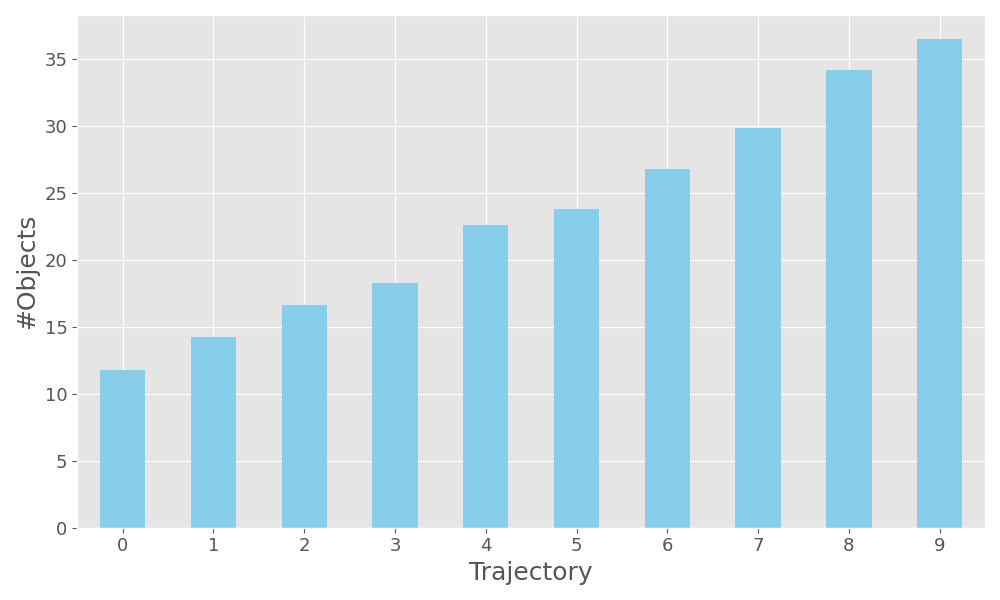
\includegraphics[width=\textwidth]{figures/10_traces/objects.png}
    \caption{Number of objects in every trajectory of $\Ttrain$ averaged among all domains.}
  \end{subfigure}
  \hfill
  \begin{subfigure}[b]{0.48\textwidth}
    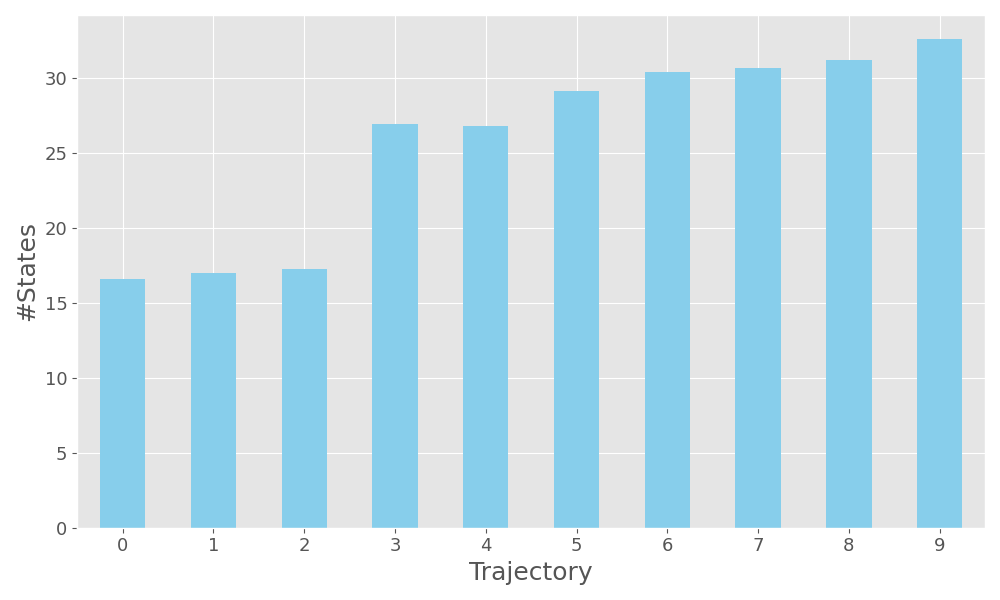
\includegraphics[width=\textwidth]{figures/10_traces/states.png}
    \caption{Number of states in every trajectory of $\Ttrain$ averaged among all domains.}
  \end{subfigure}
  
% \caption{Evaluation metric values for the models learned by \sam, \offlam, \nolam in every benchmark domain. The training set $\Ttrain$ includes $10$ trajectories for every domain.}
\end{figure} 
\vspace{4cm}
\subsection{Detailed Experimental Results}

\begin{table}[h]
\centering
\resizebox{1\columnwidth}{!}{
\begin{tabular}{l|c|c|c|c|c|c|c|c}
% \toprule
\hline
% Domain & Syn. P $\uparrow$ & Syn. R $\uparrow$ & App. P $\uparrow$ & App. R $\uparrow$ & Pred. effs. P $\uparrow$ & Pred. effs. R $\uparrow$ & Solving ratio $\uparrow$ & False plans ratio $\downarrow$ \\
Domain & \multicolumn{2}{c|}{Syntactic} & \multicolumn{2}{c|}{Applicability} & \multicolumn{2}{c|}{Predicted effects} & Solvability \% $\uparrow$ & False plans \% $\downarrow$ \\
 & \makecell[c]{P$\uparrow$} & \makecell[c]{R$\uparrow$} & \makecell[c]{P$\uparrow$} & \makecell[c] {R$\uparrow$} &  \makecell[c]{P$\uparrow$} & \makecell[c] {R$\uparrow$} & & \\
% \midrule
\hline
barman  & 0.95 $^{2}$ & 1.0 $^{1,2,3}$ & 1.0 $^{1,2,3}$ & 0.94 $^{2}$ & 1 $^{1,2,3}$ & 1 $^{1,2,3}$ & 1.0 $^{2}$ & 0 $^{1,2,3}$ \\
blocksworld  & 1.0 $^{2}$ & 1.0 $^{1,2,3}$ & 1.0 $^{1,2,3}$ & 1.0 $^{1,2,3}$ & 1 $^{1,2,3}$ & 1 $^{1,2,3}$ & 1.0 $^{1,2,3}$ & 0 $^{1,2,3}$ \\
childsnack  & 0.97 $^{2}$ & 0.9 $^{1}$ & 1.0 $^{1}$ & 1.0 $^{2}$ & 1 $^{1,2,3}$ & 1 $^{1,2,3}$ & 1.0 $^{1}$ & 0 $^{1}$ \\
depots  & 0.98 $^{2}$ & 1.0 $^{1,2,3}$ & 1.0 $^{1,2,3}$ & 1.0 $^{2}$ & 1 $^{1,2,3}$ & 1 $^{1,2,3}$ & 1.0 $^{1,2,3}$ & 0 $^{1,2,3}$ \\
elevators  & 0.81 $^{2}$ & 1.0 $^{1,2,3}$ & 1.0 $^{1,2,3}$ & 1.0 $^{2}$ & 1 $^{1,2,3}$ & 1 $^{1,2,3}$ & 1.0 $^{2}$ & 0 $^{1,2,3}$ \\
ferry  & 0.93 $^{2}$ & 1.0 $^{1,2,3}$ & 1.0 $^{1,2,3}$ & 1.0 $^{1,2,3}$ & 1 $^{1,2,3}$ & 1 $^{1,2,3}$ & 1.0 $^{1,2,3}$ & 0 $^{1,2,3}$ \\
floortile  & 0.83 $^{2}$ & 1.0 $^{1,2,3}$ & 1.0 $^{1,2,3}$ & 1.0 $^{2}$ & 1 $^{1,2,3}$ & 1 $^{1,2,3}$ & 1.0 $^{2}$ & 0 $^{1,2,3}$ \\
goldminer  & 0.8 $^{2}$ & 0.98 $^{1,2,3}$ & 1.0 $^{1,2,3}$ & 1.0 $^{2}$ & 1 $^{1,2,3}$ & 1 $^{1,2,3}$ & 1.0 $^{1,3}$ & 0 $^{1,3}$ \\
grippers  & 1.0 $^{2}$ & 1.0 $^{1,2,3}$ & 1.0 $^{1,2,3}$ & 1.0 $^{2}$ & 1 $^{1,2,3}$ & 1 $^{1,2,3}$ & 1.0 $^{1,2,3}$ & 0 $^{1,2,3}$ \\
matchingbw  & 0.95 $^{2}$ & 1.0 $^{1,2,3}$ & 1.0 $^{1,2,3}$ & 0.98 $^{1,2,3}$ & 1 $^{1,2,3}$ & 1 $^{1,2,3}$ & 1.0 $^{1,2,3}$ & 0 $^{1,2,3}$ \\
miconic  & 1.0 $^{2}$ & 1.0 $^{1,2,3}$ & 1.0 $^{1,2,3}$ & 1.0 $^{1,2,3}$ & 1 $^{1,2,3}$ & 1 $^{1,2,3}$ & 1.0 $^{1,2,3}$ & 0 $^{1,2,3}$ \\
nomystery  & 0.94 $^{2}$ & 1.0 $^{1,2,3}$ & 1.0 $^{1,2,3}$ & 1.0 $^{2}$ & 1 $^{1,2,3}$ & 1 $^{1,2,3}$ & 1.0 $^{2}$ & 0 $^{1,2,3}$ \\
npuzzle  & 0.88 $^{2}$ & 1.0 $^{1,2,3}$ & 1.0 $^{1,2,3}$ & 1.0 $^{1,2,3}$ & 1 $^{1,2,3}$ & 1 $^{1,2,3}$ & 1.0 $^{1,2,3}$ & 0 $^{1,2,3}$ \\
parking  & 0.89 $^{2}$ & 1.0 $^{1,2,3}$ & 1.0 $^{1,2,3}$ & 1.0 $^{2}$ & 1 $^{1,2,3}$ & 1 $^{1,2,3}$ & 1.0 $^{2}$ & 0 $^{1,2,3}$ \\
rovers  & 0.83 $^{2}$ & 0.93 $^{1,2,3}$ & 1.0 $^{1,2,3}$ & 1.0 $^{2}$ & 1 $^{1,2,3}$ & 1 $^{1,2,3}$ & 1.0 $^{2}$ & 0 $^{1,2,3}$ \\
satellite  & 1.0 $^{2}$ & 1.0 $^{1,2,3}$ & 1.0 $^{1,2,3}$ & 1.0 $^{2}$ & 1 $^{1,2,3}$ & 1 $^{1,2,3}$ & 1.0 $^{1,2,3}$ & 0 $^{1,2,3}$ \\
sokoban  & 0.88 $^{2}$ & 1.0 $^{1,2,3}$ & 1.0 $^{1,2,3}$ & 1.0 $^{1,2,3}$ & 1 $^{1,2,3}$ & 1 $^{1,2,3}$ & 1.0 $^{1,2,3}$ & 0 $^{1,2,3}$ \\
spanner  & 0.93 $^{2}$ & 1.0 $^{1,2,3}$ & 1.0 $^{1,2,3}$ & 1.0 $^{1,2,3}$ & 1 $^{1,2,3}$ & 1 $^{1,2,3}$ & 1.0 $^{1,2,3}$ & 0 $^{1,2,3}$ \\
tpp  & 0.95 $^{2}$ & 1.0 $^{2}$ & 1.0 $^{1,2,3}$ & 1.0 $^{2}$ & 1 $^{1,2,3}$ & 1 $^{1,2,3}$ & 1.0 $^{2}$ & 0 $^{1,2,3}$ \\
transport  & 0.93 $^{2}$ & 1.0 $^{1,2,3}$ & 1.0 $^{1,2,3}$ & 1.0 $^{1,2,3}$ & 1 $^{1,2,3}$ & 1 $^{1,2,3}$ & 1.0 $^{1,2,3}$ & 0 $^{1,2,3}$ \\
% \bottomrule
\hline
\end{tabular}
}
% \caption{Best metric values for every domain obtained among \sam, \offlam, \nolam, respectively denoted by 1,2, and 3; P indicates the precision and R the recall, $\uparrow$ (resp. $\downarrow$) denotes the higher (resp. lower) the better.}
\caption{Best metric values for every domain obtained among \sam, \offlam, \nolam, respectively denoted by 1,2, and 3; P indicates the precision and R the recall, $\uparrow$ (resp. $\downarrow$) denotes the higher (resp. lower) the better. The training set $\Ttrain$ includes $10$ trajectories for every domain.}
\end{table}

\begin{figure}[ht]
% \label{fix:exp-results}
  \centering

  \begin{subfigure}[b]{0.45\textwidth}
    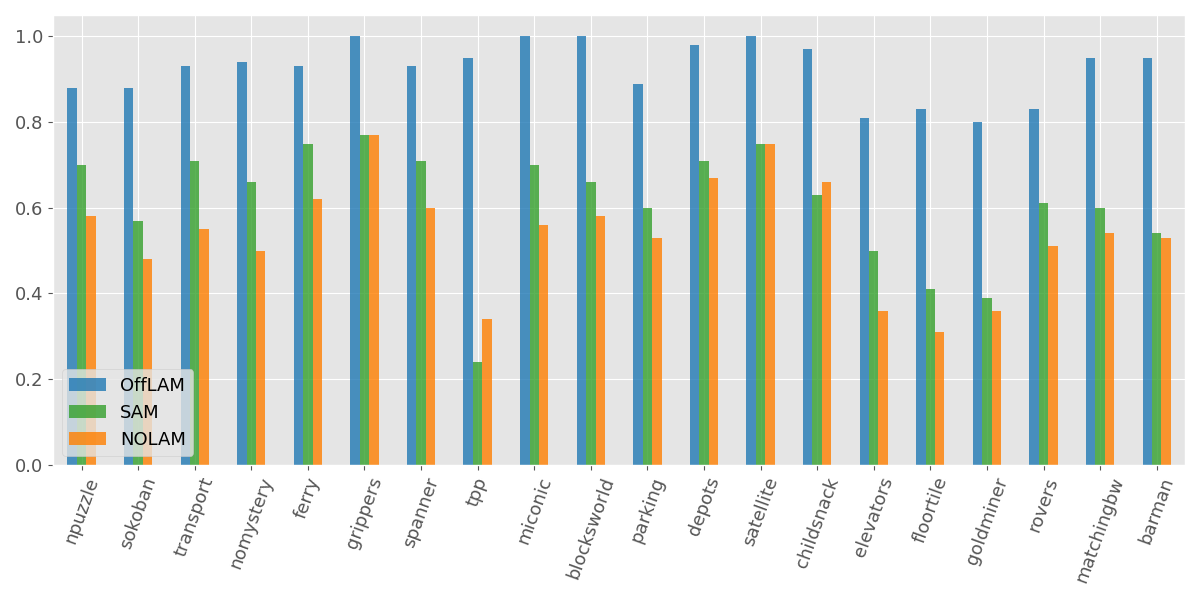
\includegraphics[width=\textwidth]{figures/10_traces/syn_precision.png}
    \caption{Syntactic precision}
  \end{subfigure}
  \hfill
  \begin{subfigure}[b]{0.45\textwidth}
    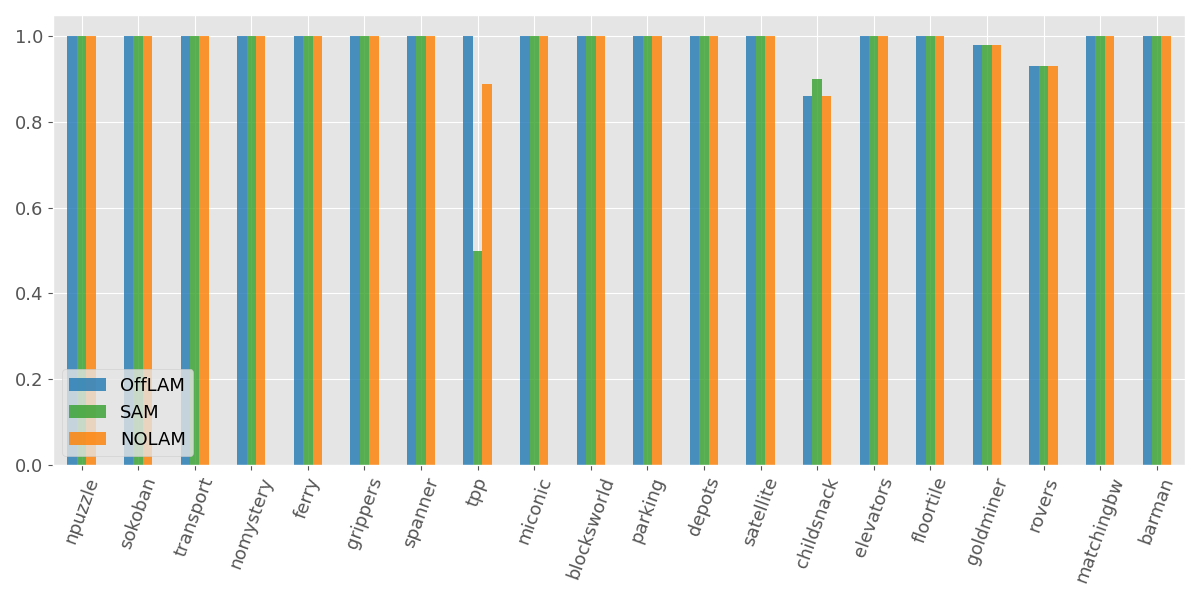
\includegraphics[width=\textwidth]{figures/10_traces/syn_recall.png}
    \caption{Syntactic recall}
  \end{subfigure}

  \vspace{1em}

  \begin{subfigure}[b]{0.45\textwidth}
    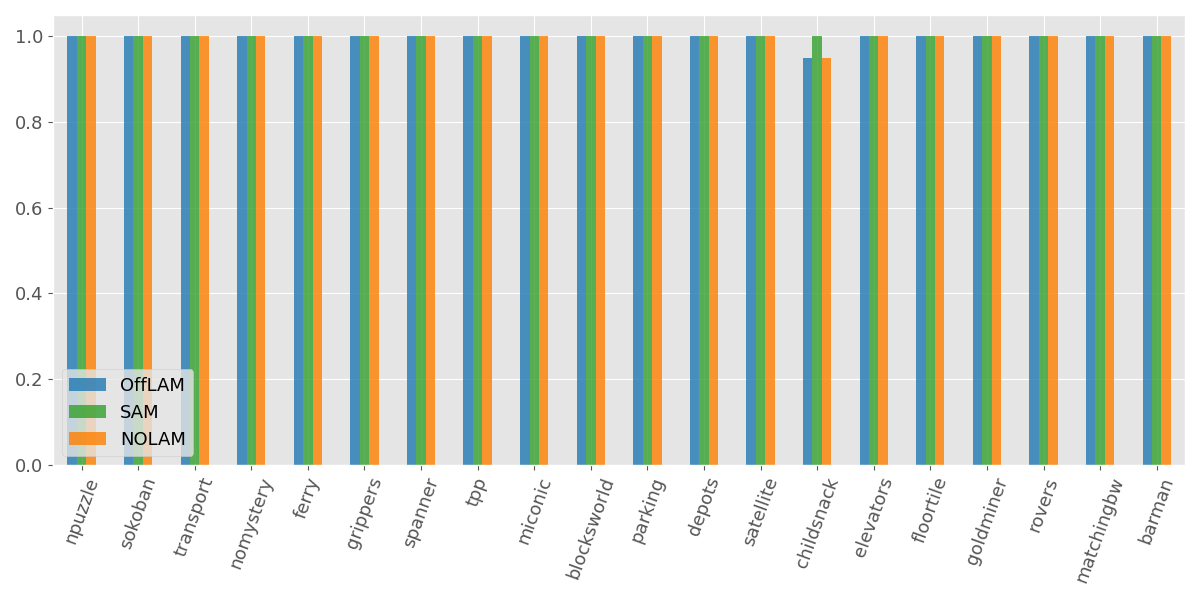
\includegraphics[width=\textwidth]{figures/10_traces/app_precision.png}
    \caption{Applicability precision}
  \end{subfigure}
  \hfill
  \begin{subfigure}[b]{0.45\textwidth}
    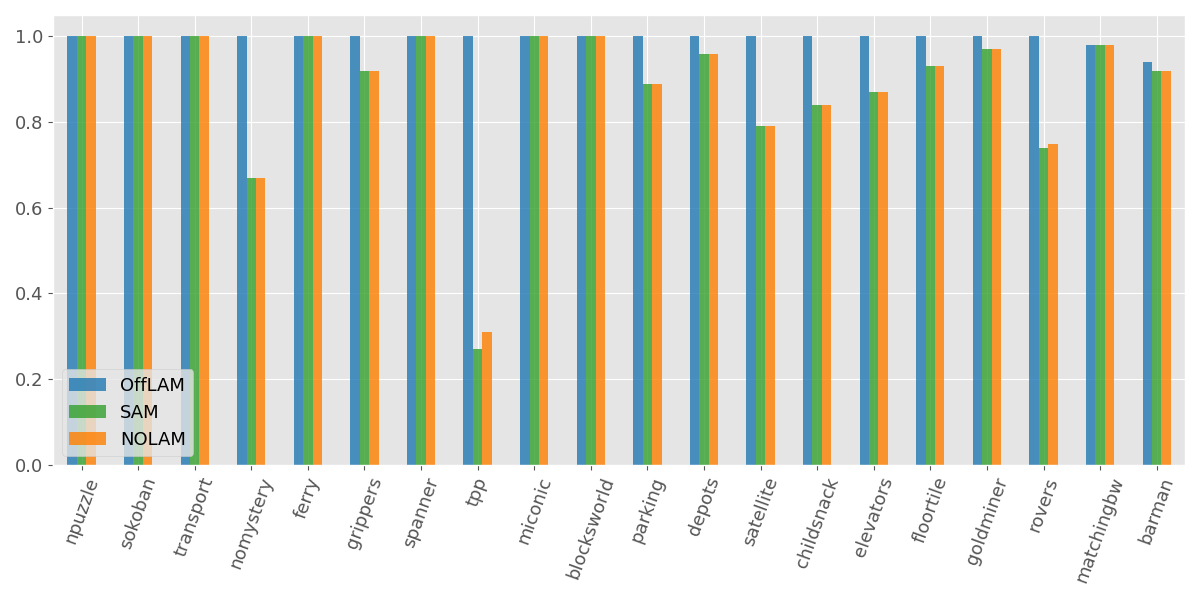
\includegraphics[width=\textwidth]{figures/10_traces/app_recall.png}
    \caption{Applicability recall}
  \end{subfigure}

  \vspace{1em}

  \begin{subfigure}[b]{0.45\textwidth}
    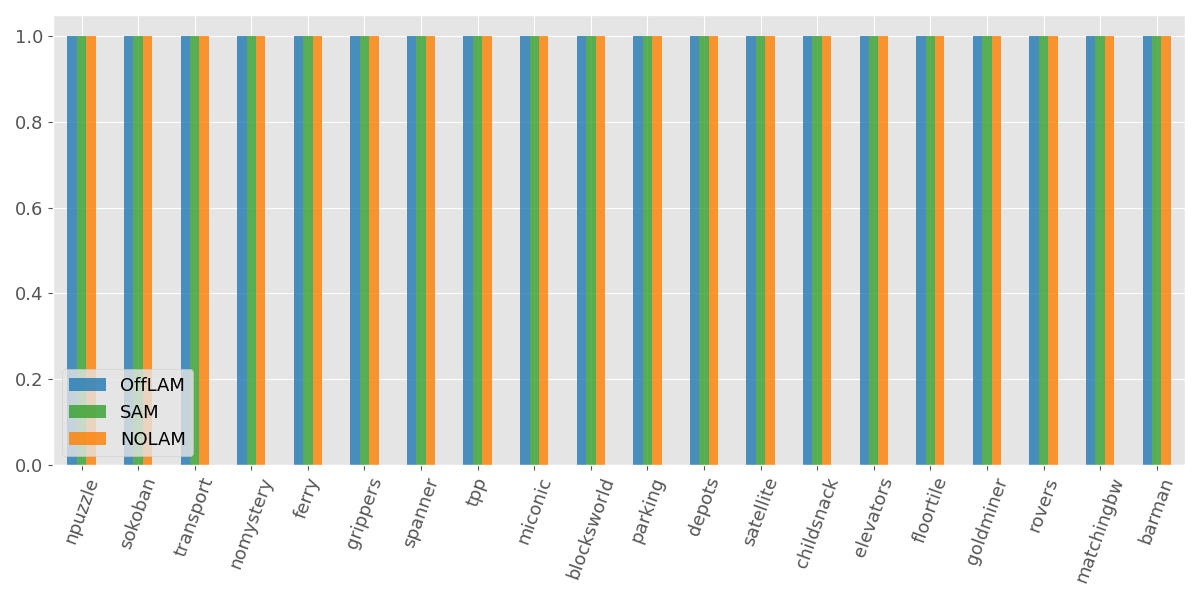
\includegraphics[width=\textwidth]{figures/10_traces/predeffs_precision.png}
    \caption{Predicted effects precision}
  \end{subfigure}
  \hfill
  \begin{subfigure}[b]{0.45\textwidth}
    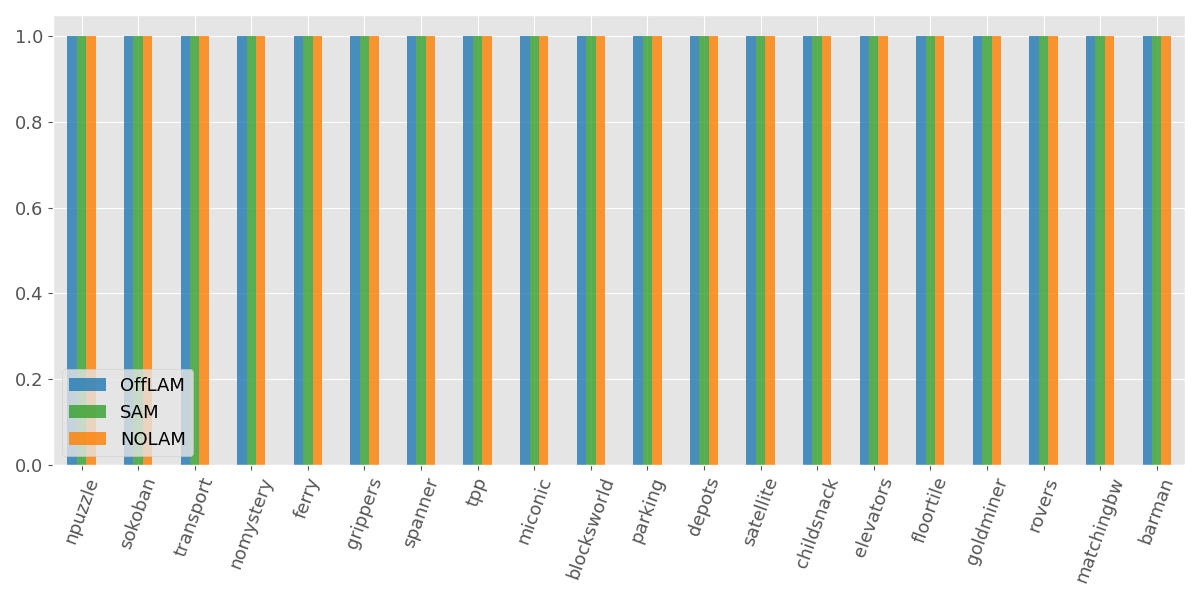
\includegraphics[width=\textwidth]{figures/10_traces/predeffs_recall.png}
    \caption{Predicted effects recall}
  \end{subfigure}

  \vspace{1em}

  \begin{subfigure}[b]{0.45\textwidth}
    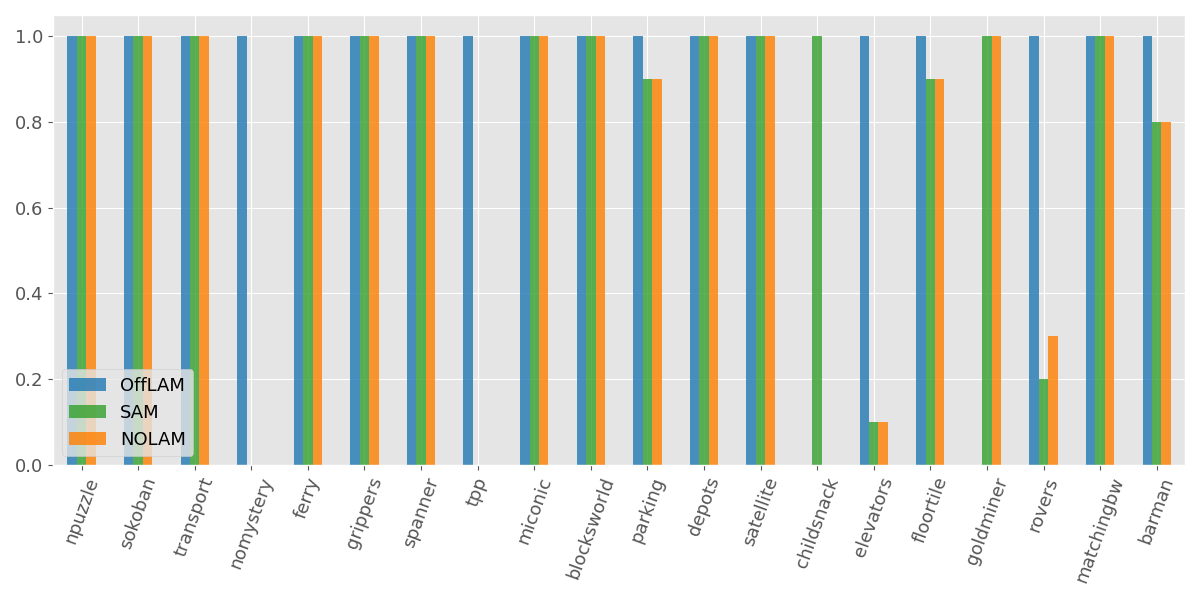
\includegraphics[width=\textwidth]{figures/10_traces/solving.png}
    \caption{Problem solving ratio}
  \end{subfigure}
  \hfill
  \begin{subfigure}[b]{0.45\textwidth}
    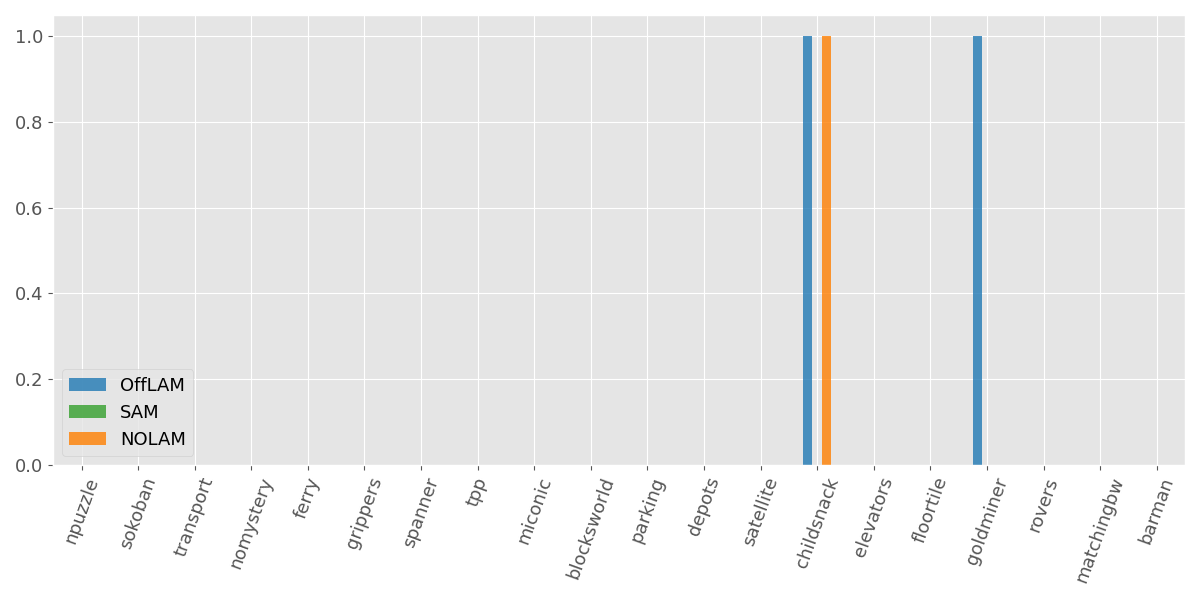
\includegraphics[width=\textwidth]{figures/10_traces/false_plans.png}
    \caption{False plans ratio}
    \label{fig:false-positive-plans}
  \end{subfigure}

  % \caption{Overall caption for the 6 images.}
  % \caption{Evaluation metrics when learning from a training set $\Ttrain$ with $10$ traces for every domain.}
\caption{Evaluation metric values for the models learned by \sam, \offlam, \nolam in every benchmark domain. The training set $\Ttrain$ includes $10$ trajectories for every domain.}
  % \label{fig:exp}
\end{figure} 
% \clearpage


\clearpage
\subsection{Additional Experimental Results}
We also conducted an additional experiments where we generated a training set $\hat{T}_{train}$ with only $2$ trajectories with $10$ states for every domain. To generate this dataset, we produced heuristic plan by considering the $2$ most complex problem settings (in terms of number of objects) adopted for generating the training set with $10$ trajectories for every domain.

\subsection{Training Set $\hat{T}_{train}$ Statistics}
\begin{table}[ht]
\centering
\resizebox{.45\columnwidth}{!}{
\begin{tabular}{l|c|c|c}
% \toprule
\hline
 Domain & \# Objects & \# States & \# Lifted Actions \\
% \midrule
\hline
barman & 33.50 & 9.00 & 10.00 \\
blocksworld & 11.50 & 9.00 & 10.00 \\
childsnack & 38.50 & 9.00 & 10.00 \\
depots & 40.50 & 9.00 & 10.00 \\
elevators & 17.50 & 9.00 & 10.00 \\
ferry & 23.00 & 9.00 & 10.00 \\
floortile & 73.00 & 9.00 & 10.00 \\
goldminer & 33.00 & 9.00 & 10.00 \\
grippers & 27.50 & 9.00 & 10.00 \\
matchingbw & 13.50 & 9.00 & 10.00 \\
miconic & 15.00 & 9.00 & 10.00 \\
nomystery & 23.50 & 9.00 & 10.00 \\
npuzzle & 49.00 & 9.00 & 10.00 \\
parking & 18.00 & 9.00 & 10.00 \\
rovers & 38.50 & 9.00 & 10.00 \\
satellite & 39.50 & 9.00 & 10.00 \\
sokoban & 107.00 & 9.00 & 10.00 \\
spanner & 32.50 & 9.00 & 10.00 \\
tpp & 24.50 & 9.00 & 10.00 \\
transport & 48.50 & 9.00 & 10.00 \\
% \bottomrule
\end{tabular}
}
\caption{Average number of states, objects, and lifted actions in the training set $\hat{T}_{train}$ with $2$ trajectories for every domain.}
% \label{tab:traj-stats}
\end{table}
\vspace{1cm}

\begin{figure}[ht!]
% \label{fix:exp-results}
  \centering

  \begin{subfigure}[b]{0.48\textwidth}
    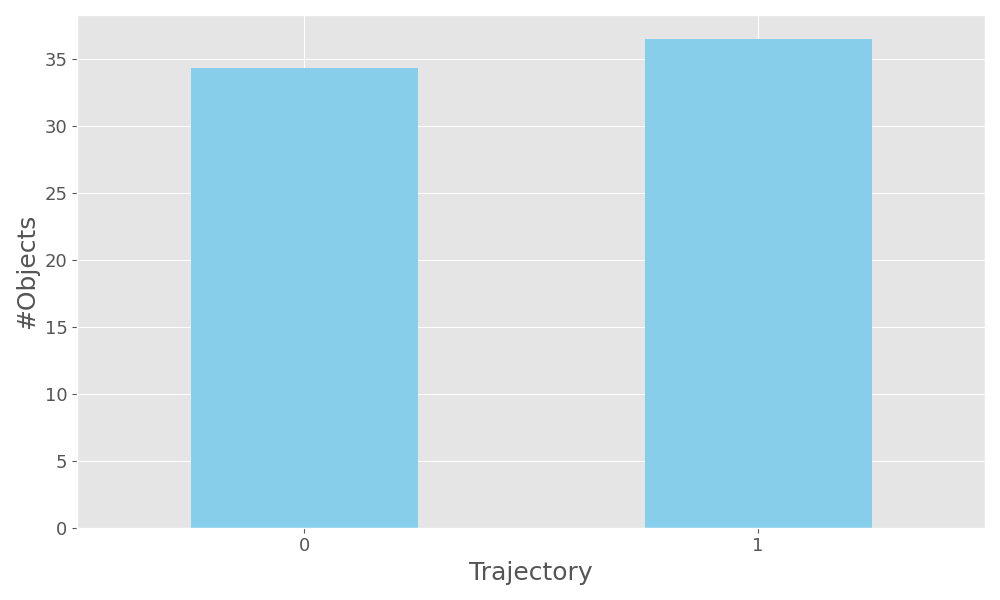
\includegraphics[width=\textwidth]{figures/2_traces/objects.png}
    \caption{Number of objects in every trajectory of $\hat{T}_{train}$ averaged among all domains.}
  \end{subfigure}
  \hfill
  \begin{subfigure}[b]{0.48\textwidth}
    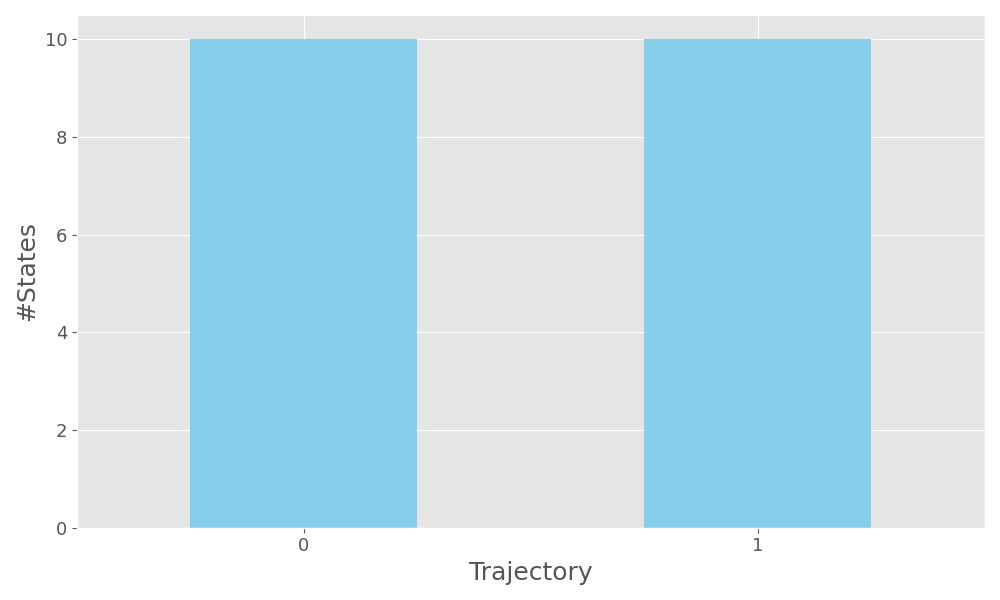
\includegraphics[width=\textwidth]{figures/2_traces/states.png}
    \caption{Number of states in every trajectory of $\hat{T}_{train}$ averaged among all domains.}
  \end{subfigure}
  
% \caption{Evaluation metric values for the models learned by \sam, \offlam, \nolam in every benchmark domain. The training set $\Ttrain$ includes $10$ trajectories for every domain.}
\end{figure} 

\begin{figure}[ht]
  \centering

  \begin{subfigure}[b]{0.45\textwidth}
    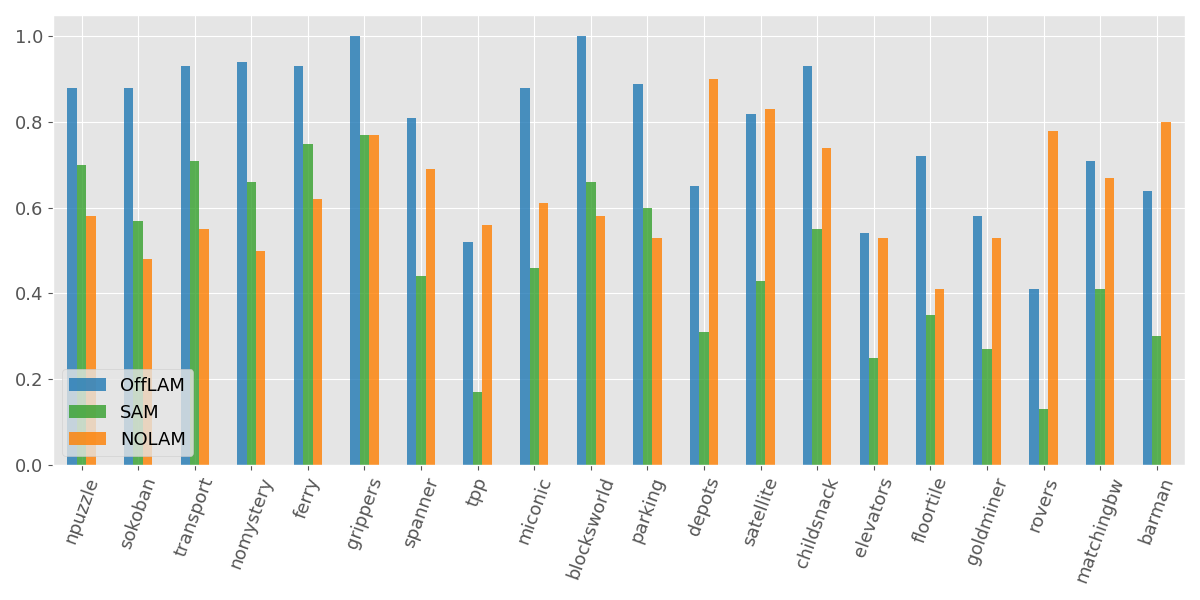
\includegraphics[width=\textwidth]{figures/2_traces/syn_precision.png}
    \caption{Syntactic precision}
  \end{subfigure}
  \hfill
  \begin{subfigure}[b]{0.45\textwidth}
    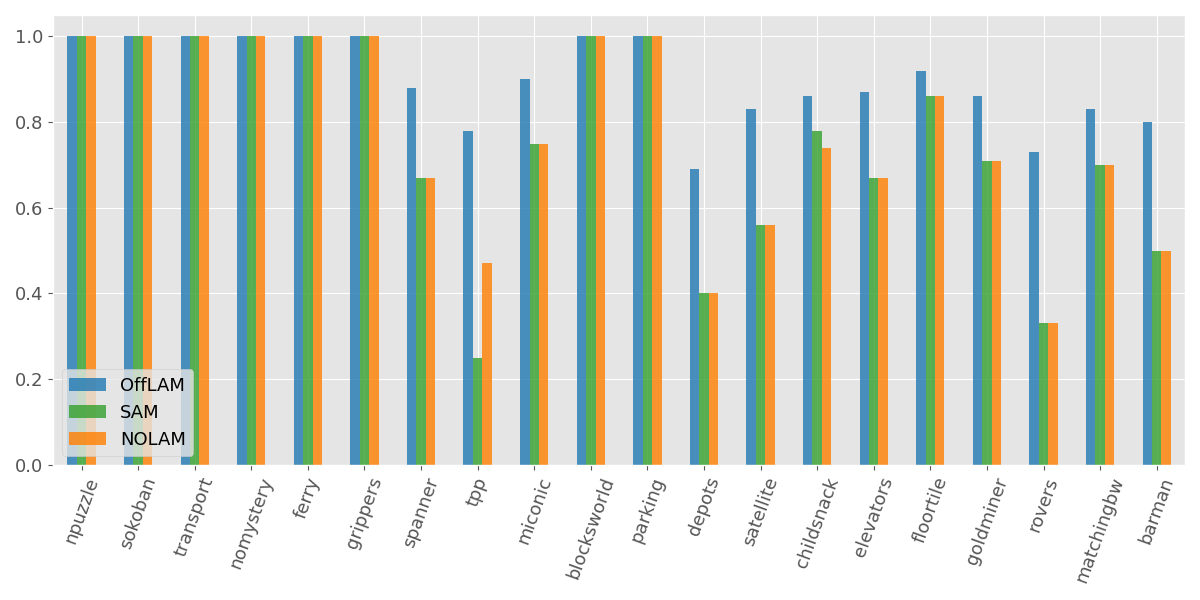
\includegraphics[width=\textwidth]{figures/2_traces/syn_recall.png}
    \caption{Syntactic recall}
  \end{subfigure}

  \vspace{1em}

  \begin{subfigure}[b]{0.45\textwidth}
    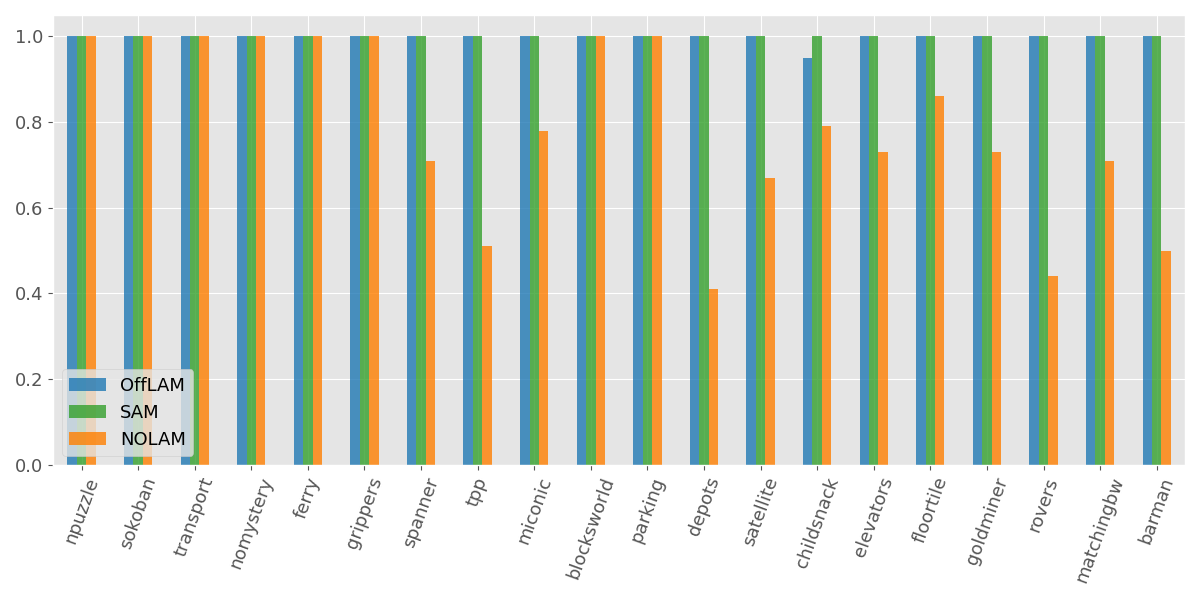
\includegraphics[width=\textwidth]{figures/2_traces/app_precision.png}
    \caption{Applicability precision}
  \end{subfigure}
  \hfill
  \begin{subfigure}[b]{0.45\textwidth}
    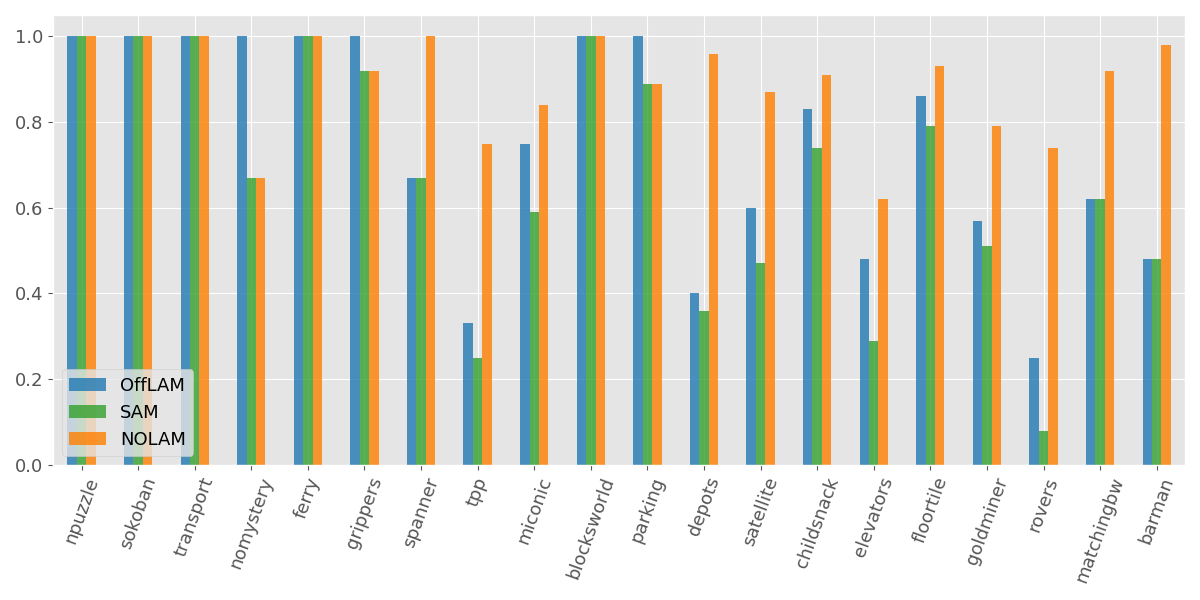
\includegraphics[width=\textwidth]{figures/2_traces/app_recall.png}
    \caption{Applicability recall}
  \end{subfigure}

  \vspace{1em}

  \begin{subfigure}[b]{0.45\textwidth}
    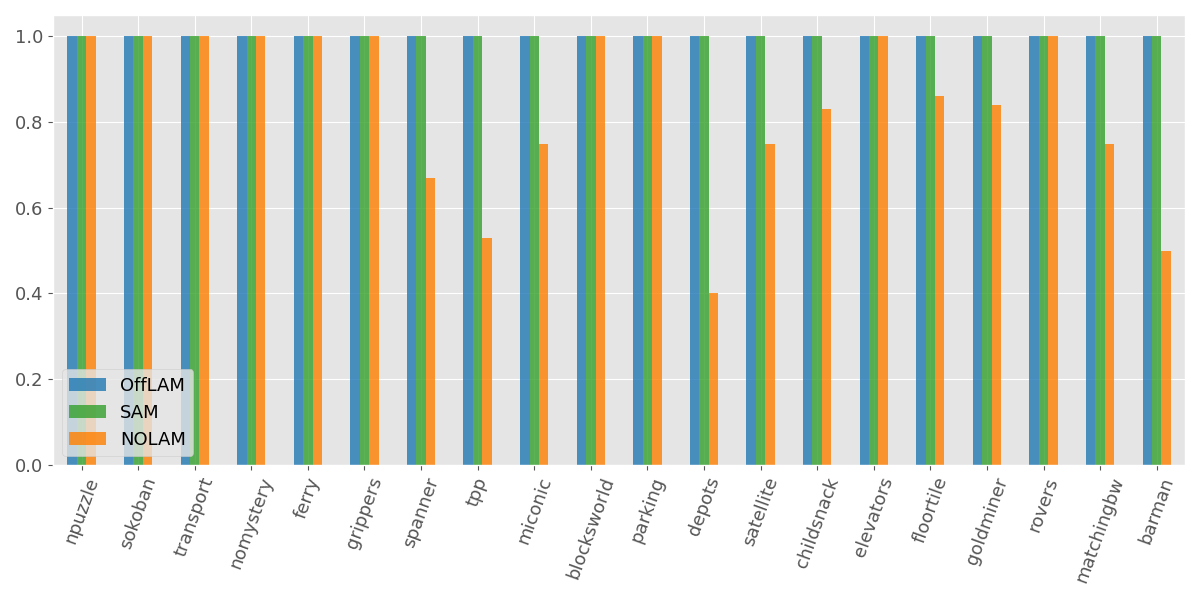
\includegraphics[width=\textwidth]{figures/2_traces/predeffs_precision.png}
    \caption{Predicted effects precision}
  \end{subfigure}
  \hfill
  \begin{subfigure}[b]{0.45\textwidth}
    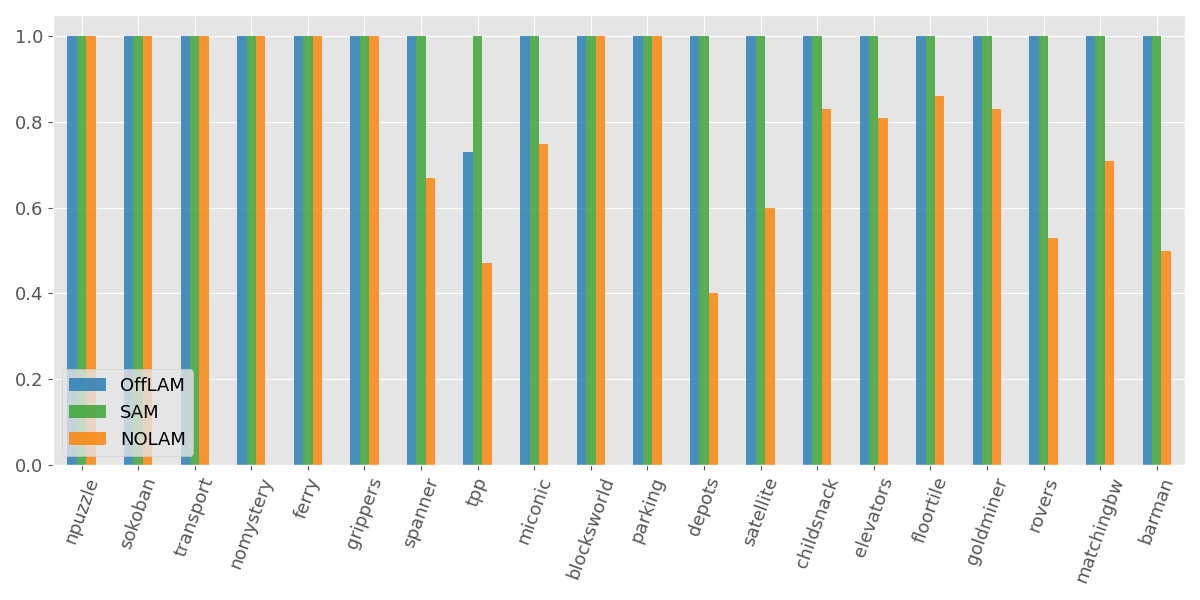
\includegraphics[width=\textwidth]{figures/2_traces/predeffs_recall.png}
    \caption{Predicted effects recall}
  \end{subfigure}

  \vspace{1em}

  \begin{subfigure}[b]{0.45\textwidth}
    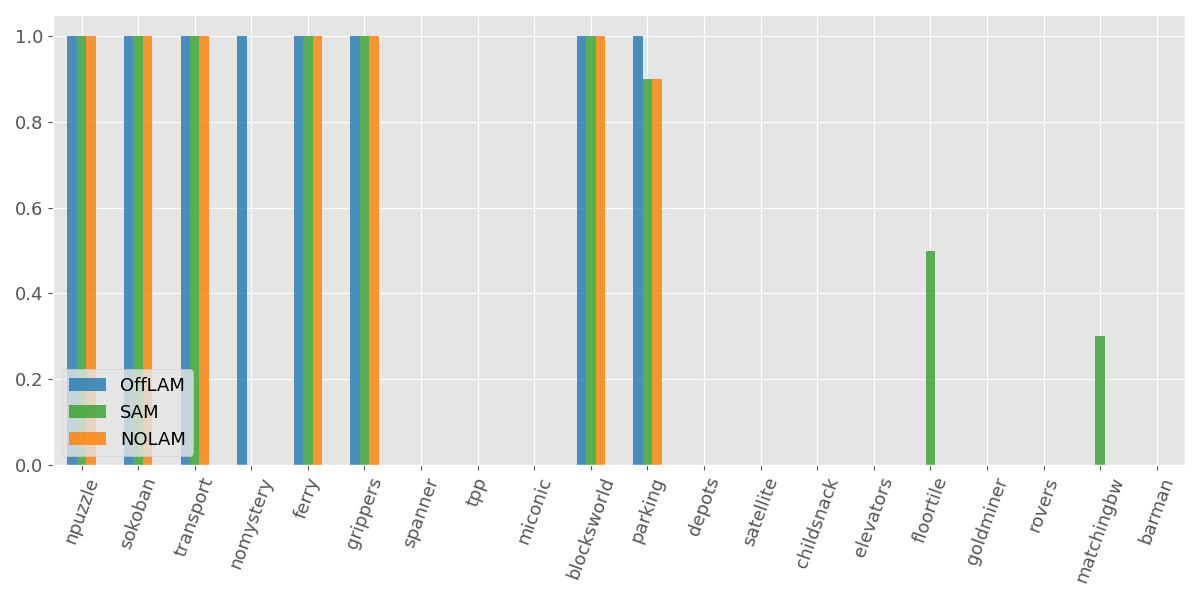
\includegraphics[width=\textwidth]{figures/2_traces/solving.png}
    \caption{Problem solving ratio}
  \end{subfigure}
  \hfill
  \begin{subfigure}[b]{0.45\textwidth}
    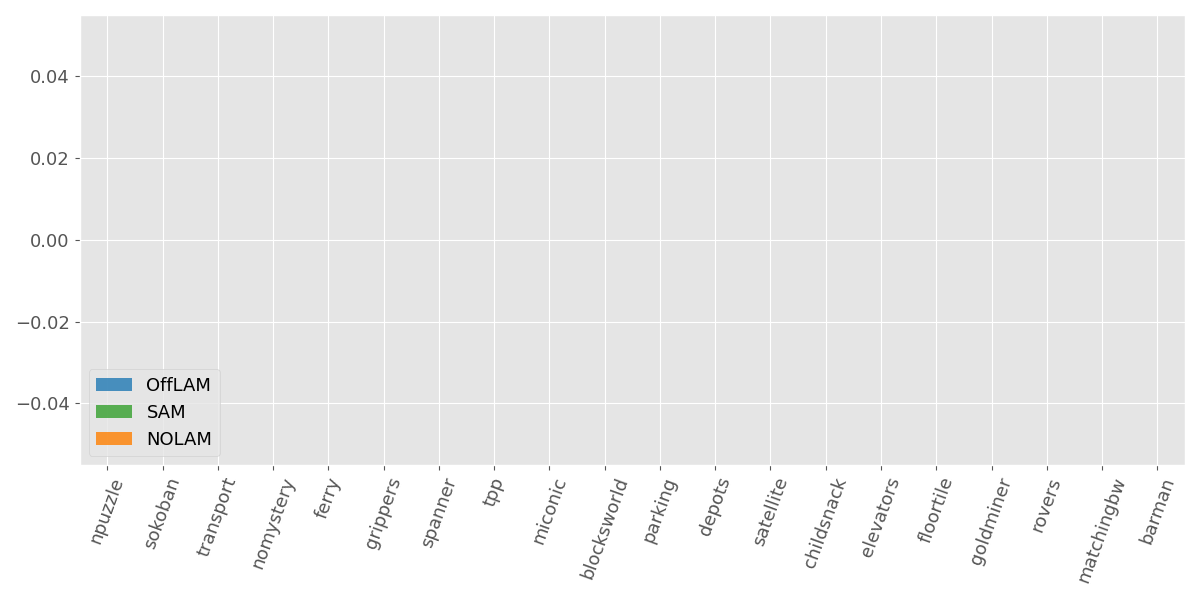
\includegraphics[width=\textwidth]{figures/2_traces/false_plans.png}
    \caption{False plans ratio}
  \end{subfigure}

  % \caption{Overall caption for the 6 images.}
  \caption{Evaluation metrics when learning from a training set $\hat{T}_{train}$ with $2$ traces for every domain.}
\end{figure} 


\begin{table}[h]
\centering
\resizebox{1\columnwidth}{!}{
\begin{tabular}{l|c|c|c|c|c|c|c|c}
% \toprule
\hline
% Domain & Syn. P $\uparrow$ & Syn. R $\uparrow$ & App. P $\uparrow$ & App. R $\uparrow$ & Pred. effs. P $\uparrow$ & Pred. effs. R $\uparrow$ & Solving ratio $\uparrow$ & False plans ratio $\downarrow$ \\
Domain & \multicolumn{2}{c|}{Syntactic} & \multicolumn{2}{c|}{Applicability} & \multicolumn{2}{c|}{Predicted effects} & Solvability \% $\uparrow$ & False plans \% $\downarrow$ \\
 & \makecell[c]{P$\uparrow$} & \makecell[c]{R$\uparrow$} & \makecell[c]{P$\uparrow$} & \makecell[c] {R$\uparrow$} &  \makecell[c]{P$\uparrow$} & \makecell[c] {R$\uparrow$} & & \\
% \midrule
\hline
barman  & 0.8 $^{3}$ & 0.8 $^{2}$ & 1.0 $^{1,2}$ & 0.99 $^{3}$ & 1.0 $^{1,2}$ & 1.0 $^{1,2}$ & 0.0 $^{1,2,3}$ & 0 $^{1,2,3}$ \\
blocksworld  & 1.0 $^{2}$ & 1.0 $^{1,2,3}$ & 1.0 $^{1,2,3}$ & 1.0 $^{1,2,3}$ & 1.0 $^{1,2,3}$ & 1.0 $^{1,2,3}$ & 1.0 $^{1,2,3}$ & 0 $^{1,2,3}$ \\
childsnack  & 0.93 $^{2}$ & 0.86 $^{2}$ & 1.0 $^{1}$ & 0.91 $^{3}$ & 1.0 $^{1,2}$ & 1.0 $^{1,2}$ & 0.0 $^{1,2,3}$ & 0 $^{1,2,3}$ \\
depots & 0.9 $^{3}$ & 0.69 $^{2}$ & 1.0 $^{1,2}$ & 0.96 $^{3}$ & 1.0 $^{1,2}$ & 1.0 $^{1,2}$ & 0.0 $^{1,2,3}$ & 0 $^{1,2,3}$ \\
elevators  & 0.54 $^{2}$ & 0.87 $^{2}$ & 1.0 $^{1,2}$ & 0.63 $^{3}$ & 1.0 $^{1,2,3}$ & 1.0 $^{1,2}$ & 0.0 $^{1,2,3}$ & 0 $^{1,2,3}$ \\
ferry  & 0.93 $^{2}$ & 1.0 $^{1,2,3}$ & 1.0 $^{1,2,3}$ & 1.0 $^{1,2,3}$ & 1.0 $^{1,2,3}$ & 1.0 $^{1,2,3}$ & 1.0 $^{1,2,3}$ & 0 $^{1,2,3}$ \\
floortile & 0.72 $^{2}$ & 0.92 $^{2}$ & 1.0 $^{1,2}$ & 0.93 $^{3}$ & 1.0 $^{1,2}$ & 1.0 $^{1,2}$ & 0.5 $^{1}$ & 0 $^{1,2,3}$ \\
goldminer  & 0.58 $^{2}$ & 0.86 $^{2}$ & 1.0 $^{1,2}$ & 0.78 $^{3}$ & 1.0 $^{1,2}$ & 1.0 $^{1,2}$ & 0.0 $^{1,2,3}$ & 0 $^{1,2,3}$ \\
grippers  & 1.0 $^{2}$ & 1.0 $^{1,2,3}$ & 1.0 $^{1,2,3}$ & 1.0 $^{2}$ & 1.0 $^{1,2,3}$ & 1.0 $^{1,2,3}$ & 1.0 $^{1,2,3}$ & 0 $^{1,2,3}$ \\
matchingbw  & 0.71 $^{2}$ & 0.83 $^{2}$ & 1.0 $^{1,2}$ & 0.92 $^{3}$ & 1.0 $^{1,2}$ & 1.0 $^{1,2}$ & 0.3 $^{1}$ & 0 $^{1,2,3}$ \\
miconic  & 0.88 $^{2}$ & 0.9 $^{2}$ & 1.0 $^{1,2}$ & 0.83 $^{3}$ & 1.0 $^{1,2}$ & 1.0 $^{1,2}$ & 0.0 $^{1,2,3}$ & 0 $^{1,2,3}$ \\
nomystery  & 0.94 $^{2}$ & 1.0 $^{1,2,3}$ & 1.0 $^{1,2,3}$ & 1.0 $^{2}$ & 1.0 $^{1,2,3}$ & 1.0 $^{1,2,3}$ & 1.0 $^{2}$ & 0 $^{1,2,3}$ \\
npuzzle  & 0.88 $^{2}$ & 1.0 $^{1,2,3}$ & 1.0 $^{1,2,3}$ & 1.0 $^{1,2,3}$ & 1.0 $^{1,2,3}$ & 1.0 $^{1,2,3}$ & 1.0 $^{1,2,3}$ & 0 $^{1,2,3}$ \\
parking  & 0.89 $^{2}$ & 1.0 $^{1,2,3}$ & 1.0 $^{1,2,3}$ & 1.0 $^{2}$ & 1.0 $^{1,2,3}$ & 1.0 $^{1,2,3}$ & 1.0 $^{2}$ & 0 $^{1,2,3}$ \\
rovers  & 0.78 $^{3}$ & 0.73 $^{2}$ & 1.0 $^{1,2}$ & 0.73 $^{3}$ & 1.0 $^{1,2,3}$ & 1.0 $^{1,2}$ & 0.0 $^{1,2,3}$ & 0 $^{1,2,3}$ \\
satellite  & 0.83 $^{3}$ & 0.83 $^{2}$ & 1.0 $^{1,2}$ & 0.85 $^{3}$ & 1.0 $^{1,2}$ & 1.0 $^{1,2}$ & 0.0 $^{1,2,3}$ & 0 $^{1,2,3}$ \\
sokoban  & 0.88 $^{2}$ & 1.0 $^{1,2,3}$ & 1.0 $^{1,2,3}$ & 1.0 $^{1,2,3}$ & 1.0 $^{1,2,3}$ & 1.0 $^{1,2,3}$ & 1.0 $^{1,2,3}$ & 0 $^{1,2,3}$ \\
spanner & 0.81 $^{2}$ & 0.88 $^{2}$ & 1.0 $^{1,2}$ & 1.0 $^{3}$ & 1.0 $^{1,2}$ & 1.0 $^{1,2}$ & 0.0 $^{1,2,3}$ & 0 $^{1,2,3}$ \\
tpp  & 0.56 $^{3}$ & 0.78 $^{2}$ & 1.0 $^{1,2}$ & 0.75 $^{3}$ & 1.0 $^{1,2}$ & 1.0 $^{1}$ & 0.0 $^{1,2,3}$ & 0 $^{1,2,3}$ \\
transport  & 0.93 $^{2}$ & 1.0 $^{1,2,3}$ & 1.0 $^{1,2,3}$ & 1.0 $^{1,2,3}$ & 1.0 $^{1,2,3}$ & 1.0 $^{1,2,3}$ & 1.0 $^{1,2,3}$ & 0 $^{1,2,3}$ \\
% \bottomrule
\hline
\end{tabular}
}
% \caption{Best metric values for every domain obtained among \sam, \offlam, \nolam, respectively denoted by 1,2, and 3; P indicates the precision and R the recall, $\uparrow$ (resp. $\downarrow$) denotes the higher (resp. lower) the better.}
\caption{Best metric values for every domain obtained among \sam, \offlam, \nolam, respectively denoted by 1,2, and 3; P indicates the precision and R the recall, $\uparrow$ (resp. $\downarrow$) denotes the higher (resp. lower) the better. The training set $\hat{T}_{train}$ includes $2$ trajectories for every domain.}
\end{table}
}

% RONI: I HOPE YOU ALSO SLEEP SOMETIME ;)

% Yes soon I think.. But you too

% I'm close to converging also, but I want to submit a first version before. Close to it. 
% One thing if we're "talking" to note: I changed the flow a bit in the experimental results so its something like: (1) here's a general way to evaluate model learningn using our metrics, (2) and here's how we impelmented it ( putting here all the details like the planner configuration and all that). I already did this change, just writing so  you're not surprised or annoyed when you read it (after sleeping of course). Hope that's Ok?

% Awesome sure, thanks for saying it (but I think I would not realized it), so I am also converging with the supplementary material (and additional exp with 2 traces), tomorrow morning will polish the code so that we can submit also that

% SOUNDS Great (need to figure out how to anonymize it, but I know there are ways to do it)

% Yes i usually upload the git repo zip by removing the ".git" folder (whichh stores e.g. commit with username etc.)

% Super! TNX

% you too and good night :)